\chapter{Implementation and Realization}
The discussed approach is brought into existence in this sophisticated test environment by accessing MicroMoPS and its peripherals, by extending the pre-developed MicroMoPS firmware and by effectively utilizing the Actor framework of SAM. 
The implementation of the proposed approach is done for a Low Voltage stress test system. 
The boards that are associated with the Low voltage stress test system (\cref{fig:combination}) are termed in the MoPS environment as follows:
\begin{itemize}
	\item Application module - BuckMoPS
	\item DUT module - LGA771
\end{itemize}

%\begin{figure}
%		\centering
%		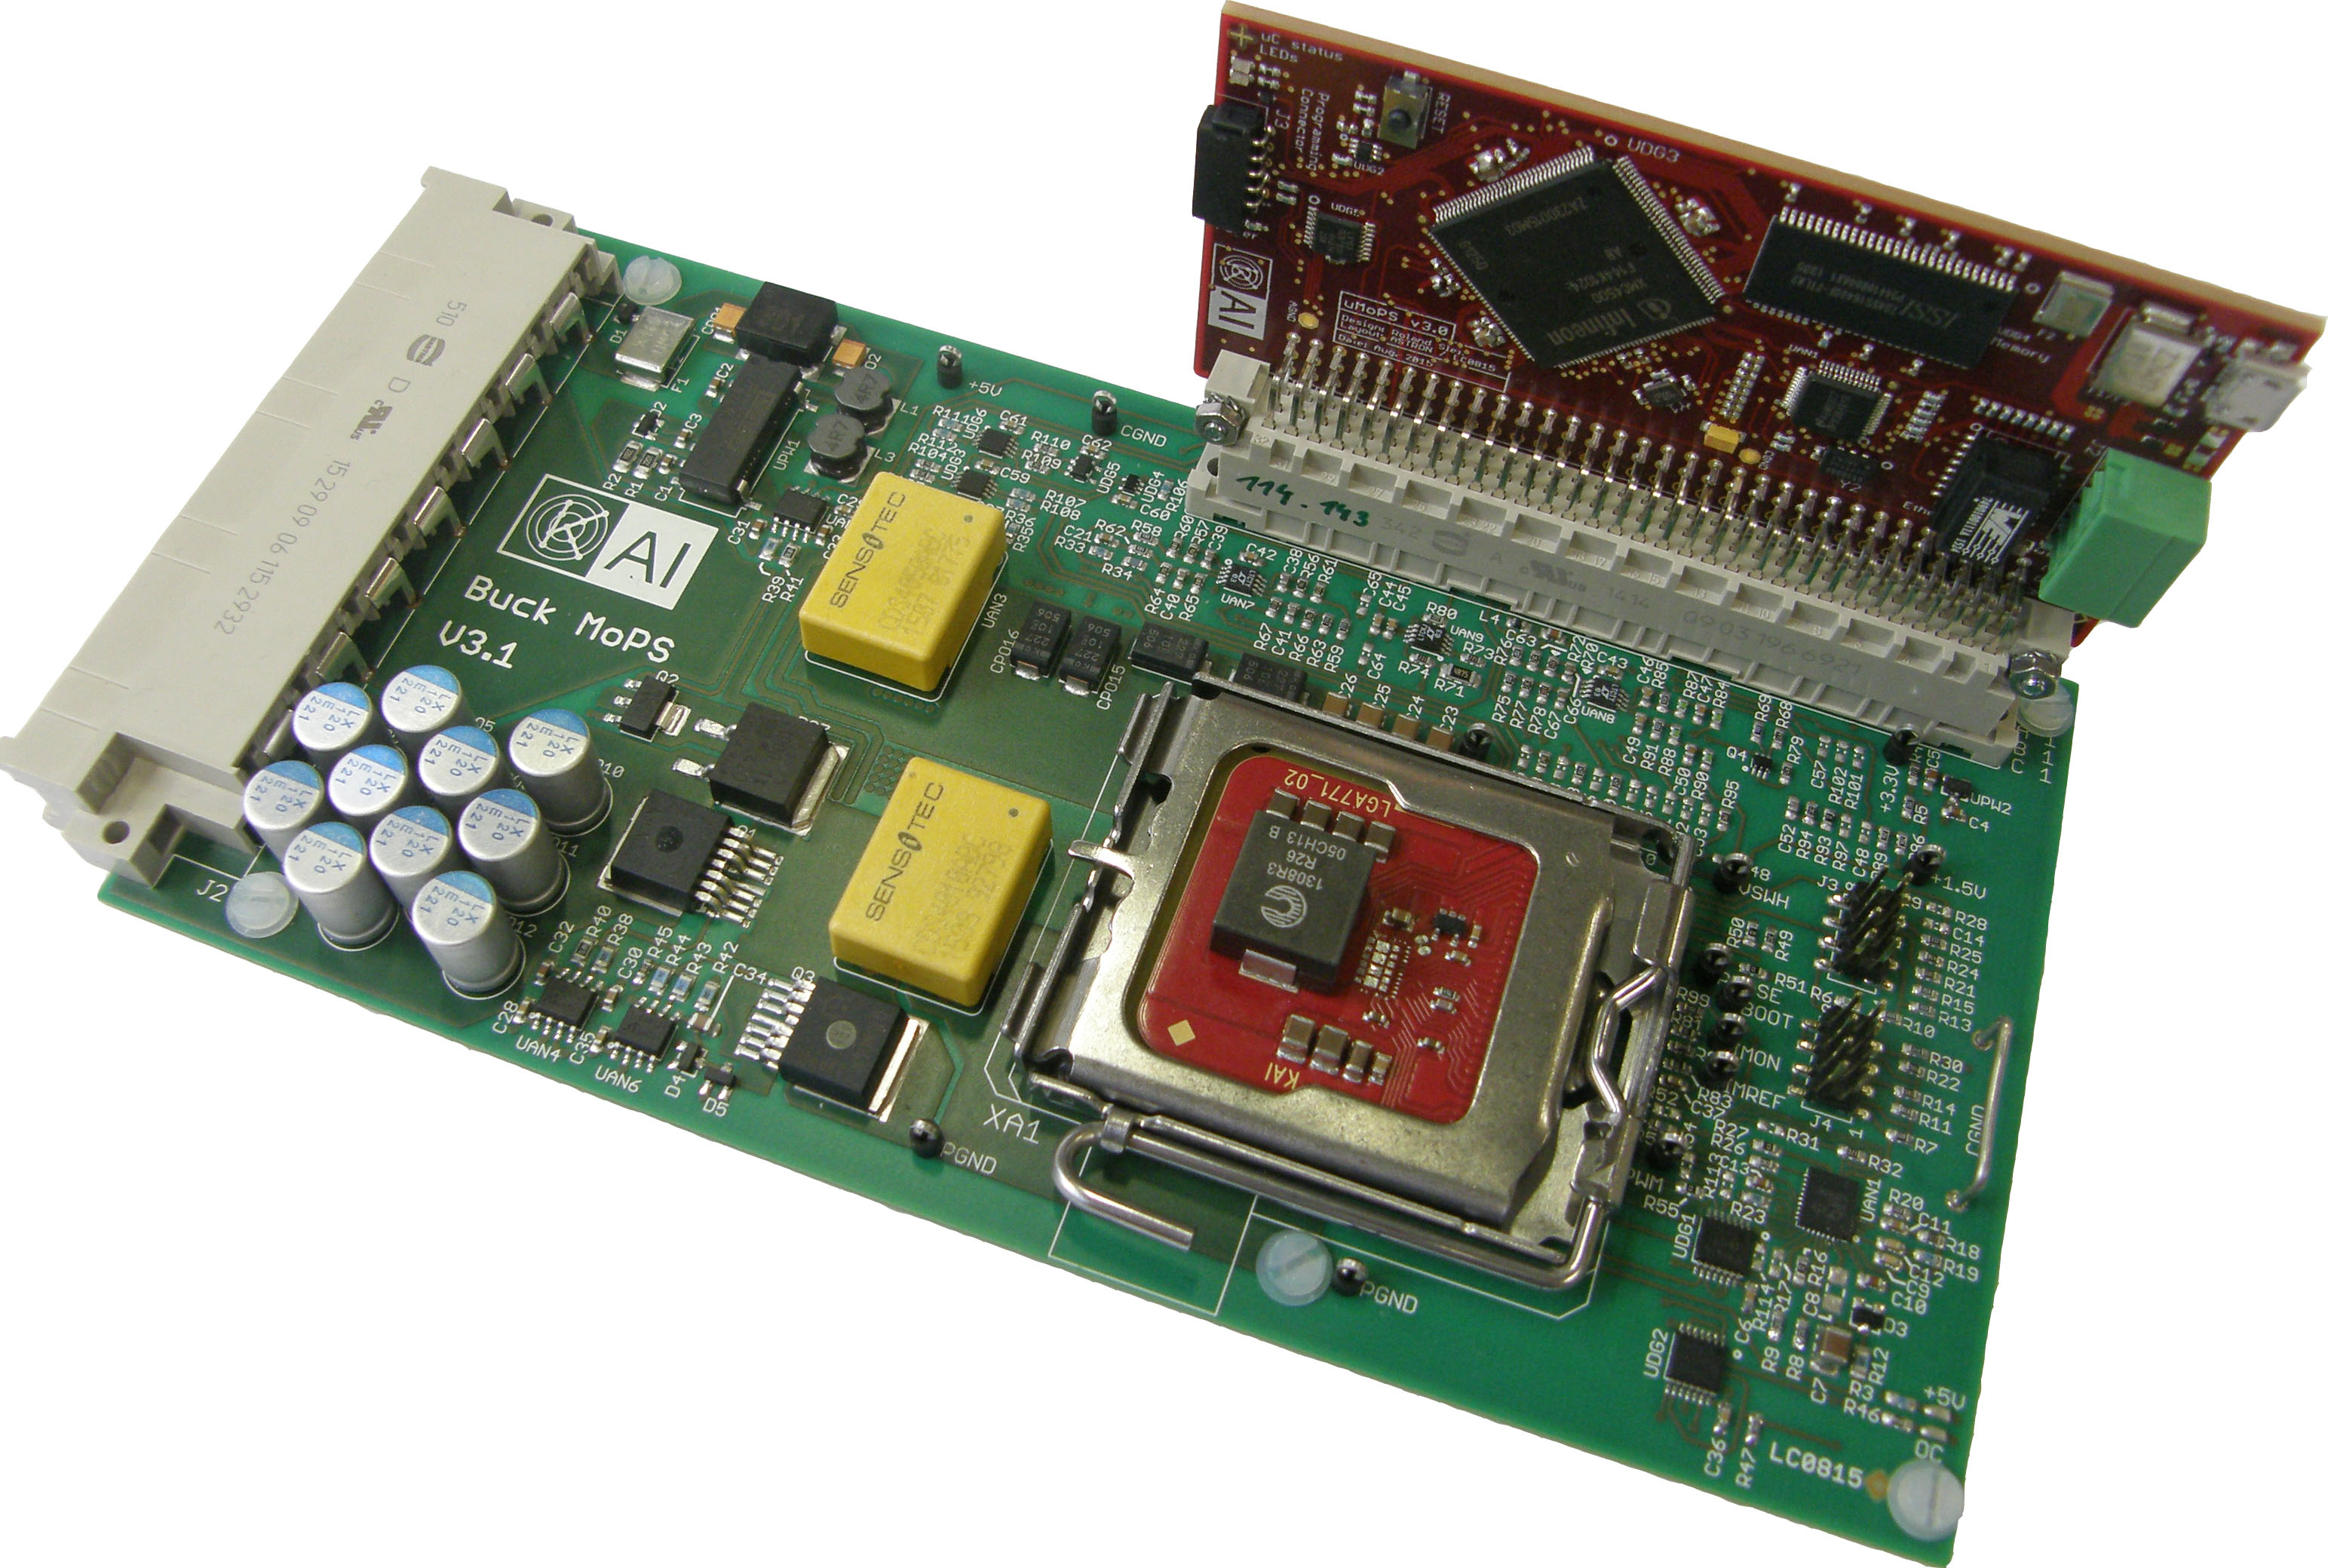
\includegraphics[trim=0 0 0 0, clip, width=100mm, scale=0.75]{images/Buck_and_uMoPS_2.jpg}
%		\caption{MicroMoPS, BuckMoPS and LGA771 arrangement.}
%		\label{combination}
%\end{figure}

\section{Extraction of UID of DUT and application board}\label{comm}
Board IDs are selected by using relevant \gls{GPIO} pins of MicroMoPS, which are meant for I2C (see \cref{sec:IIC}) communication.
In this work, MicroMoPS is treated as a Master block, DS28CM00~\cite{Maxim-DS28CM00-2006a} UID chip of application module and DUT as slave modules.
The operation of reading the board UID is succeeded by initializing and utilizing accordingly the appropriate digital IO pin of MicroMoPS.
The digital pin corresponding to the Master Module is set to appropriate mode at the very beginning of the operation.
Setting digital pin into an appropriate mode drives the Serial interface clock input (SCL) (see \cref{sec:IIC}).
Two PCA9515A~\cite{PCA951A-2014} ICs are embedded in the BuckMoPS to facilitate the MicroMoPS in reading UID of application board and \acrshort{DUT} module. 
With the support of PCA9515A ICs and UID chip, the corresponding DUT and application module are interacted from MicroMoPS using I2C communication. 

Obtainment of the board IDs is primarily controlled as per the programmer's requirement by utilizing the select line of the UIN chip of BuckMoPS. 
PCA9515A ICs are part of UIN chip present in BuckMoPS, which facilitates accessing the DS28CM00 module.
When the select line is set as logic $0$, PCA9515A of application module is enabled, which further establishes communication between MicroMoPS and UID chip of application module. 
Application module's UID can be requested using this communication. 
Similarly, when the select line is chosen as logic $1$, PCA9515A of DUT is enabled, which further establishes communication between MicroMoPS and UID chip of \acrshort{DUT}. 
\gls{DUT}'s \acrshort{UID} can be requested using this communication. 
There are two communication lines which need to be synchronously used by the master to write to UID chip or read from UID chip. 
They are, \acrshort{SDA} and \acrshort{SCL} lines (see \cref{sec:IIC}). 
SDA line is used for sending the data from master to slave or receiving the data from slave to master and SCL is used for providing synchronization in communication between master and slave. 
Because the concern is to read the board id of DUT and application module from MicroMoPS, systematic sequential communication procedure is followed (see \cref{sec:IIC}).
The received data is CRC verified using standard 8-bit polynomial i.e X8 + X5 + X4 + 1 \cite{Maxim-DS28CM00-2006a}, to authenticate the corruption of received data.

The above operation is implemented inside the test\_identify\_boards() handler (see \cref{sec:CORE}) of MicroMoPS firmware to successfully extract the board UID of BuckMoPS and LGA771.

The board \glspl{UID} extracted from slave devices are listed in the \cref{Table4}:

\begin{table}[ht]
	\centering
	\caption{Boards and their respective UID}
	\label{Table4}
	\begin{tabular}{|p{2.3cm}||p{3cm}|p{3.5cm}|p{2cm}| }
		\hline
		\textbf{Board type} &\textbf{Board name}   &\textbf{Unique Identity Number}    &\textbf{Select line}\\
		\hline
		Application module	&BuckMoPS   & 0x0d8d3c7   &0 \\
		Device under test &LGA771   	& 0x1052523   &1\\
		\hline
	\end{tabular}
\end{table}

\section{Update the microcontroller's configuration file for linear scaling computation}\label{resn}
The configuration file of a MicroMoPS contains the initializations of MicroMoPS associated peripheral modules. 
These modules are configurable based on the firmware developer's needs.
In the MicroMoPS firmware project, there is a dedicated configuration file to manage the configurations of a MicroMoPS called "config.c".

%\section{Update the configuration of MicroMoPS to integrate linear scaling mechanism.}\label{sec:configuration file}

%Could be included in implementation section
%Mathematically, obtained linear scaling mechanism is incorporated to processing of analog measurements in MicroMoPS, by updating the configuration of MicroMoPS. Scaling dependent structure in the configuration file of MicroMoPS is updated by appending linear scaling parameters for every communication channels of MicroMoPS. Updating, the configuration intuitively means that linear scaling variables can be used for digital data processing via a firmware module. EDS is also generated upon microcontroller booting (see Section\cref{CORE})

To incorporate the linear scaling mechanism to MicroMoPS, the scaling module i.e MoPS scaling, is extended by adding two parameters as shown in the \cref{lst:code_scaling}.
The added parameters are \emph{scaling factor} and \emph{offset} in adjacent to the respective analog channel (.name) parameter.
The scaling values that are assigned are the default scaling values.
These values are meaningful to measurement circuits of the Low-Voltage stress test system.
These scaling values are updated automatically with different values when the stress test system that is performed is different from the Low-Voltage test system.

The \gls{EDS} is generated every time when the MicroMoPS firmware starts. 
The EDS contains the communication channels and channels' specific scaling parameters. 
The \acrshort{DUT} creation in the mops web server based on the EDS information and downloading of the \glspl{LUT} when SAM starts running was carried out by summer students of KAI.

%\begin{listing}[htp]
%	\inputminted[frame=single]{C}{src/scaling.c}
%	\caption{MoPS scaling}
%	\label{lst:code_scaling}
%\end{listing}

\lstinputlisting[frame=single, label=lst:code_scaling, caption=MoPS scaling, firstnumber=1]{src/scaling.c}

\section{Board UIDs communication to SAM}
		 The byte-wise data of \gls{UID}, which are received from the \gls{UID} chip is collected and combined inside test\_identify\_boards() (see \cref{sec:CORE}) handler to reproduce UID (64-bit length) of the board. 
		 In this work, UID of BuckMoPS and LGA771 are restored.
		 The restored UIDs are further communicated to SAM using the dedicated MicroMoPS' test handlers~\cite{Steinwender2016}.

\section{Resolution of UIDs in SAM and scaling values communication from SAM to MicroMoPS}
The resolution of Board IDs in SAM is implemented by utilizing the LabVIEW software packages. 
\begin{figure}[hbt]
		\centering
		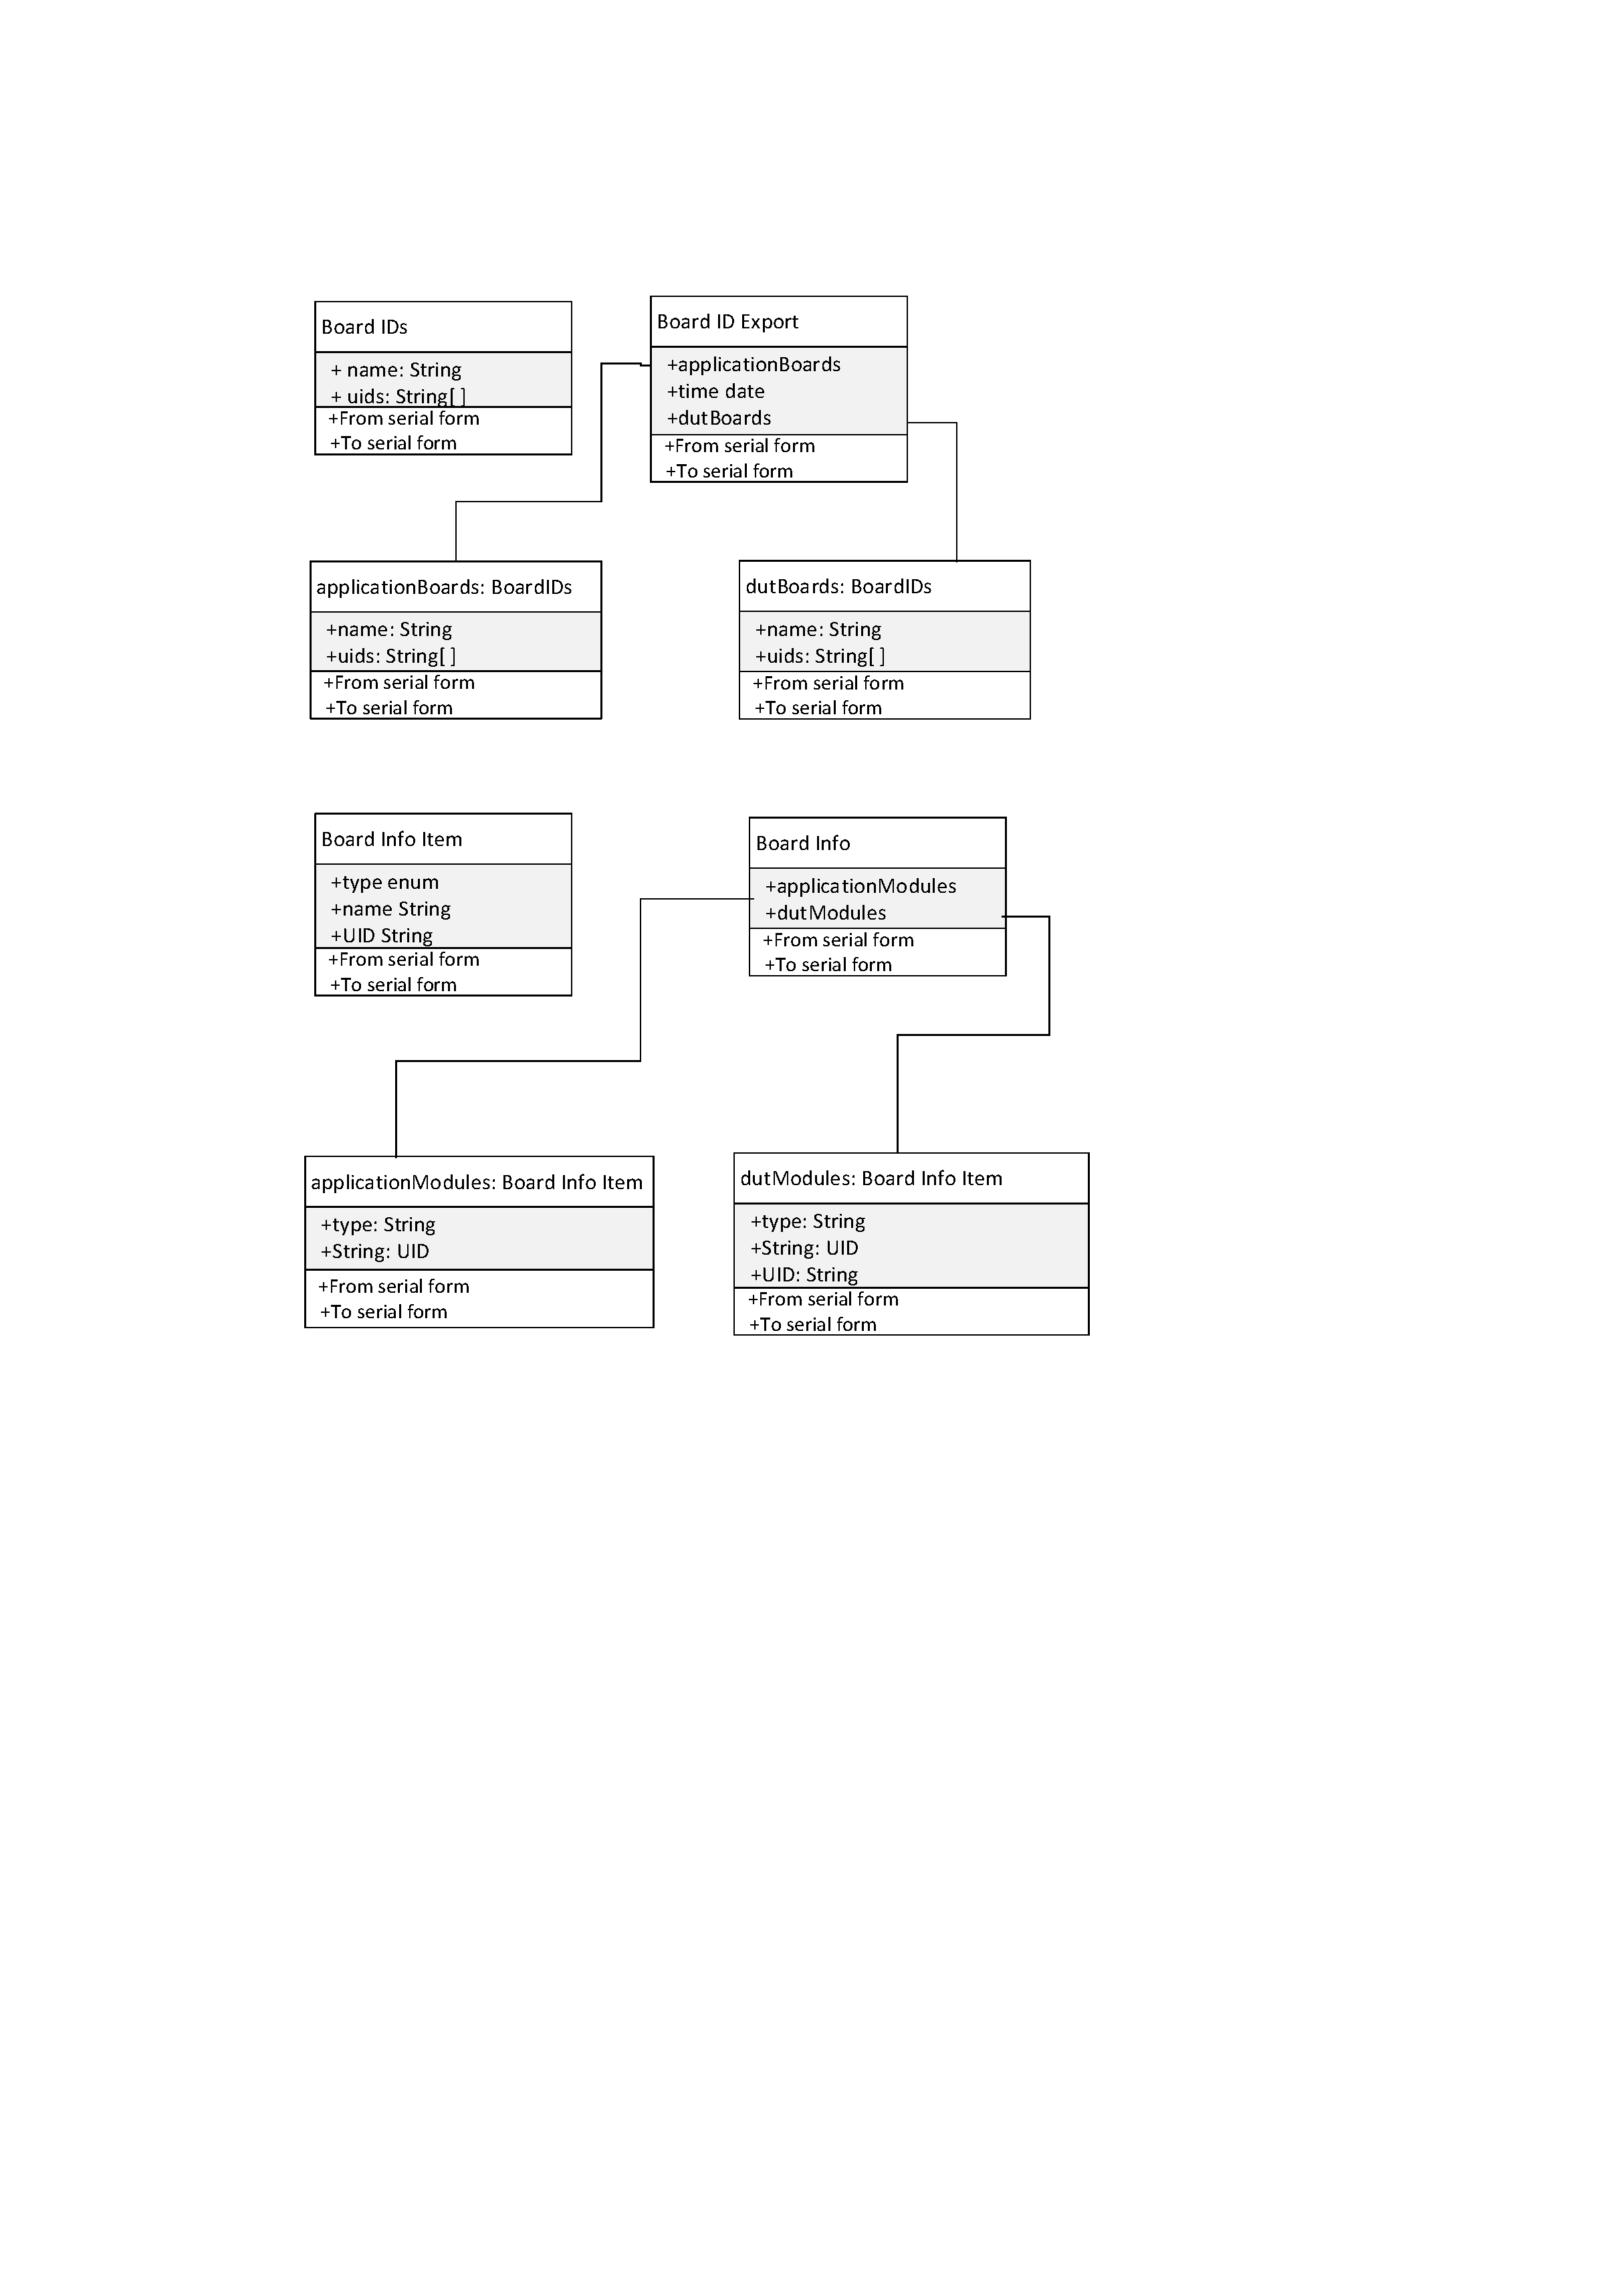
\includegraphics[trim=180 670 0 140, clip, width=210mm, scale=0.75]{images/board_objects.pdf}
		\caption{Serialization of JSON objects into LabVIEW data structures}
		\label{fig:Serialization}
\end{figure}
The basic step before the implementation of the algorithm which mainly resolves the board ids is the serialization of the application module's objects and dutBoard's objects into LabVIEW data structures as shown in the \cref{fig:Serialization}.
The application module's objects and the dutBoard's objects are present in the "boards.json".
The board UIDs are cached offline using I2C communication and communicated to SAM.
The derived scaling values and board UIDs are stored in a database of \acrshort{MoPS} web server.
As described in the \cref{sec:uidResolution}, the board database, and scaling database are downloaded by SAM from the MoPS web server. 
Intuitively, "boards.json" and "scaling.json" are downloaded by the main actor of SAM to facilitate the board UIDs resolution. 
The resolution of board UIDs is done in the Node actor (see \cref{sec:SAM}) of SAM. 
To achieve board UIDs resolution, variables such as "name" and "uids" are declared as string and array of string data members of class "Board IDs", respectively as shown in the \cref{fig:Serialization}. 
Similarly, variables such as applicationBoards and dutBoards are declared as data members of "Board ID export" class.
The data members of "Board ID export" i.e applicationBoards and dutBoards, are an instance of the class "Board IDs".
%The serialization of the JSON objects i.e application module and dutboard, is to unflatten the lists present in these JSON objects into LabVIEW variants.

The classes that are created by the name "Board IDs" and "Board ID export" are the LabVIEW classes.
The serialization methods that are present in the classes do the conversion of JSON objects present in "boards.json" into strings. 
These strings are nothing but the key-value pair of applicationModule and dutBoard as shown in the \cref{lst:boards}. 
Thus, by means of serialization, the board name and uid values of applicationModule JSON object and dutBoard JSON object are assigned to applicationBoards and dutBoards data members of "Board ID export", respectively.
In the same way, the board UIDs along with their directional pin that are received by SAM from MicroMoPS, are assigned to data members of "Board Info item".
Based on the directional pin value, the received board UIDs are classified into appropriate board type and accordingly, the board UIDs are assigned to UID data member of "Board Info item".
After a successful serialization, the UIDs of data members (applicationBoards and dutBoards) of "Board Info item" are compared with the UID of data members (applicationModules and dutModules) of "Board ID export".

\begin{figure}[hbt]
		\centering
		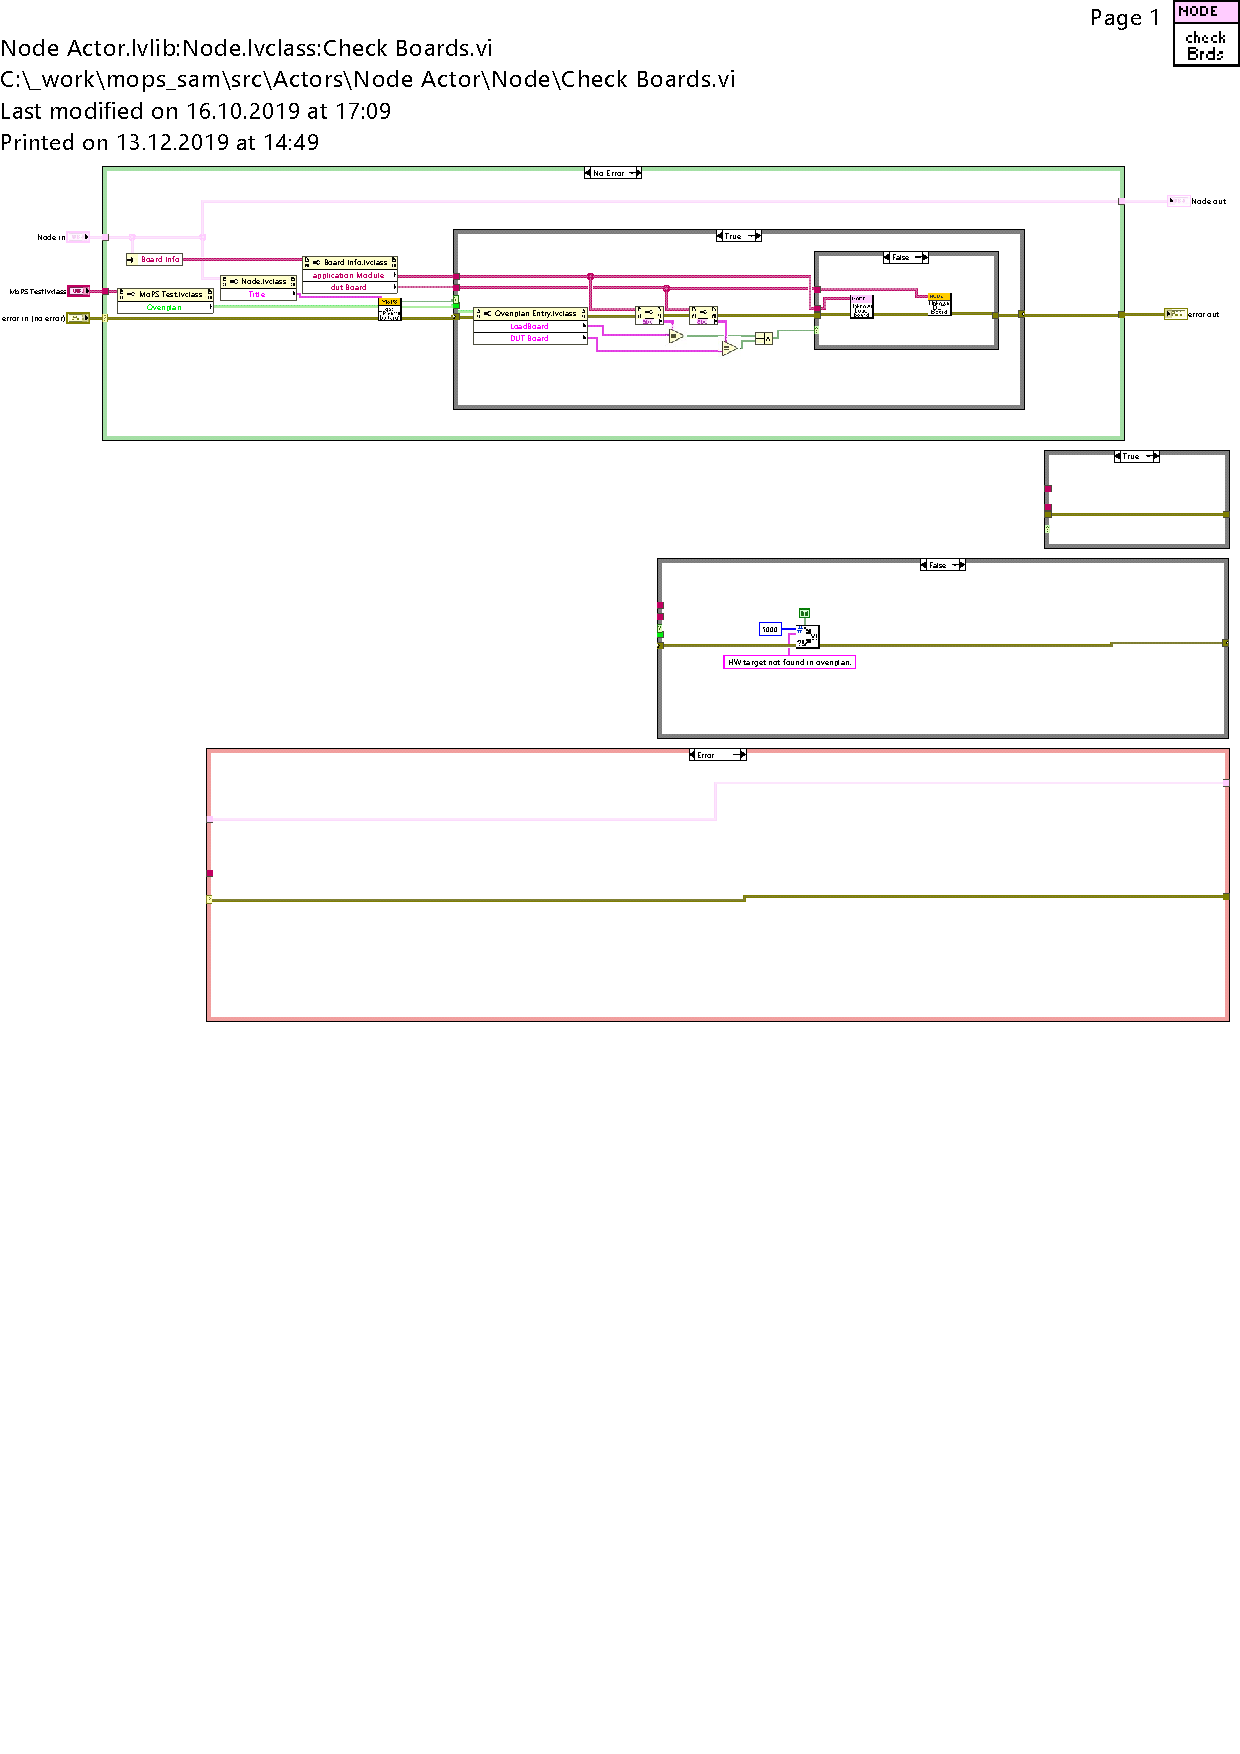
\includegraphics[trim=0 628 0 80, clip, width=155mm, height=70mm, scale=3]{images/verify.pdf}
		\caption{Verification of boards with oven plan entry.}
		\label{fig:Verify}
\end{figure}

This, comparison if found matched, the respective board names such as BuckMoPS and LGA771 are updated to application module and dutModule objects which are instances of "Board Info". 
Earlier to this update, only a UID information and the type was known to application module and dutModule objects, through the MicroMoPS communication. 
Successful comparison leads to the resolution of board UIDs. The updated board names along with their respective types in "Board Info" are logged on to the log GUI display of SAM.
Logging of board names with their type helps the test engineers or SAM developers to know the status of detection of boards by SAM.
%Explain algorithm in steps

\begin{figure}[hbt]
		\centering
		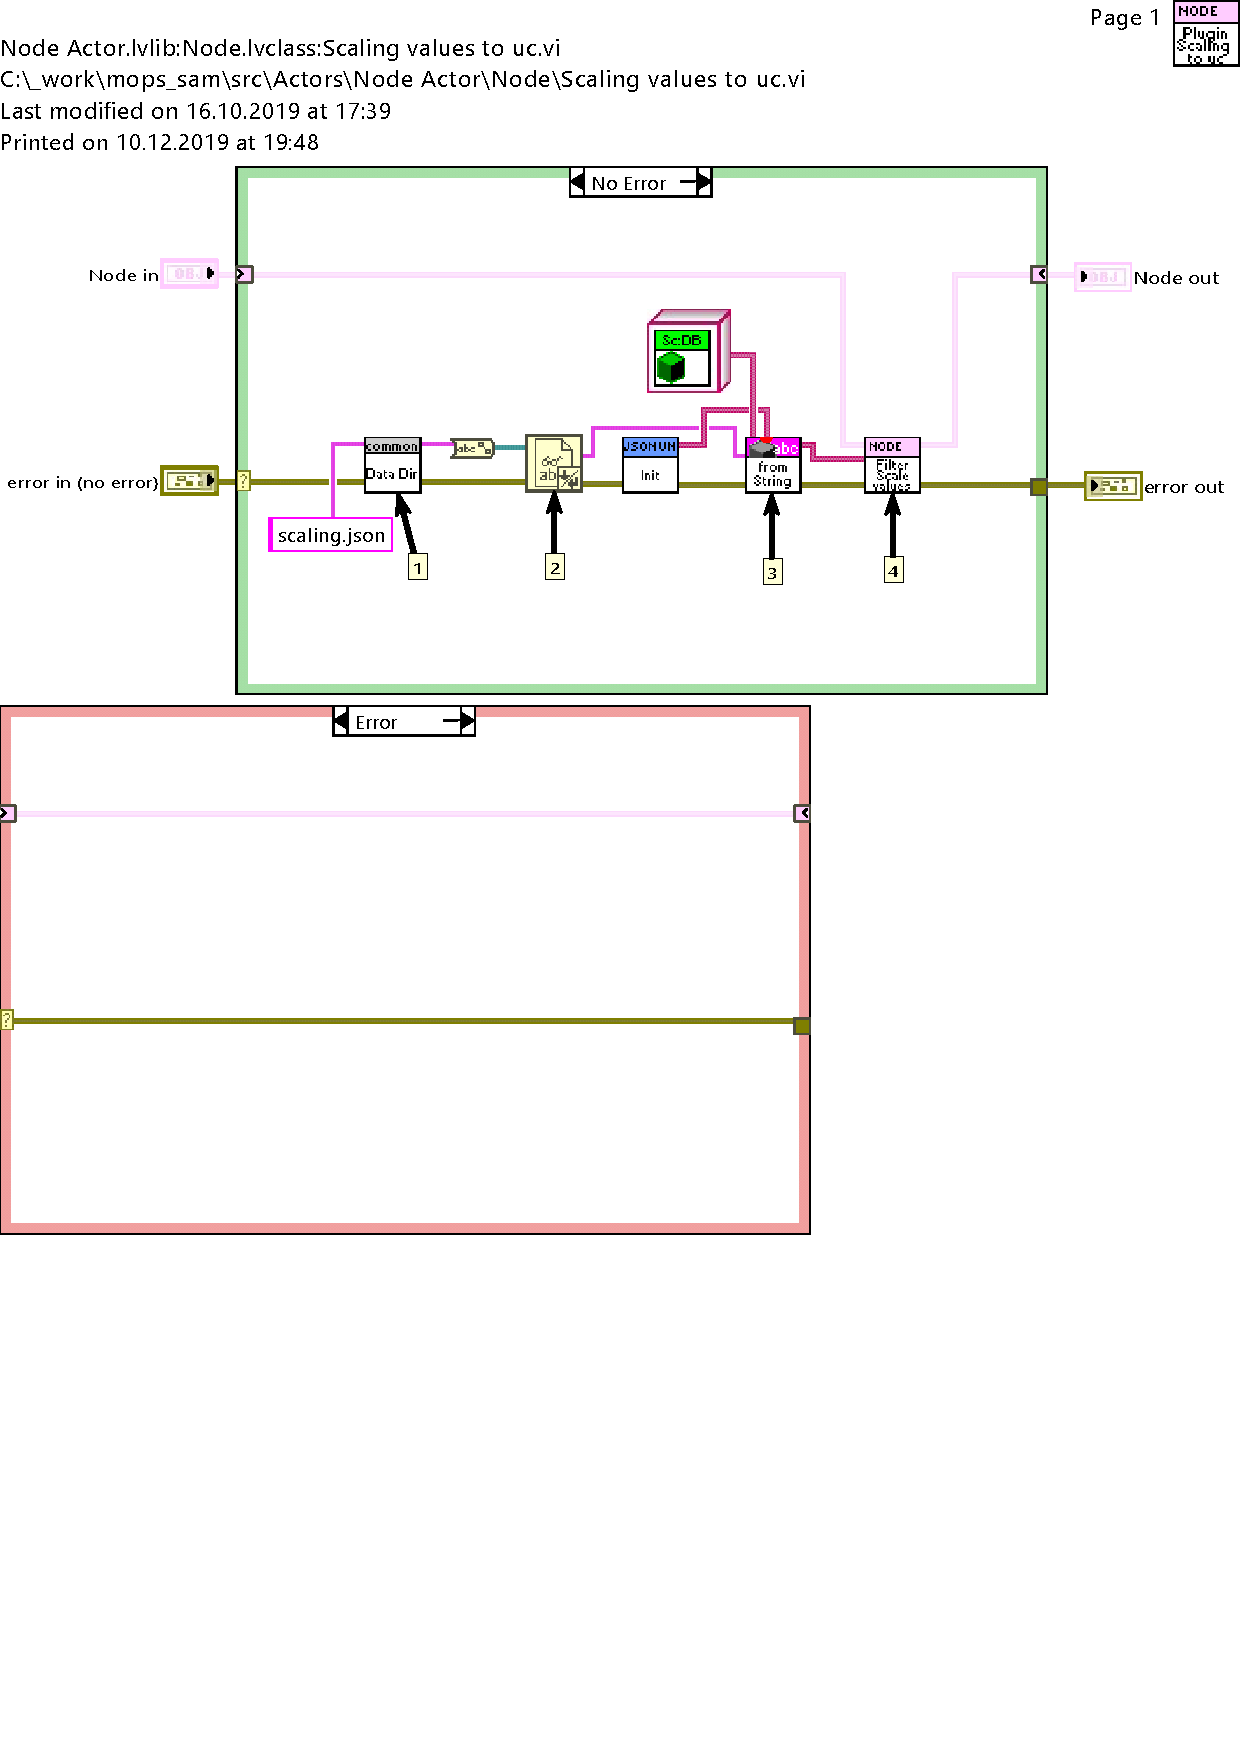
\includegraphics[trim=0 505 0 75, clip, width=150mm, scale=2]{images/Filterscalingvalues.pdf}
		\caption{Communication of channel name and associated scaling values to MicroMoPS.}
		\label{fig:Communication}
\end{figure}

Further, the board names that are present in the application module and dutModule objects are verified with the Hardware information present in the oven plan as shown in the \cref{fig:Verify}. 
The Serialization procedure as described earlier is undergone by test plan (JSON) to un-flatten the oven plan JSON objects into LabVIEW data structures. 
The Hardware information which is present in the oven plan entry class (due to serialization) is verified with the board names that are present in the application modules and dutModules.
If the verification is unsuccessful, the conflicting board information is reported to the MoPS web server. 

\begin{figure}[hbt]
		\centering
		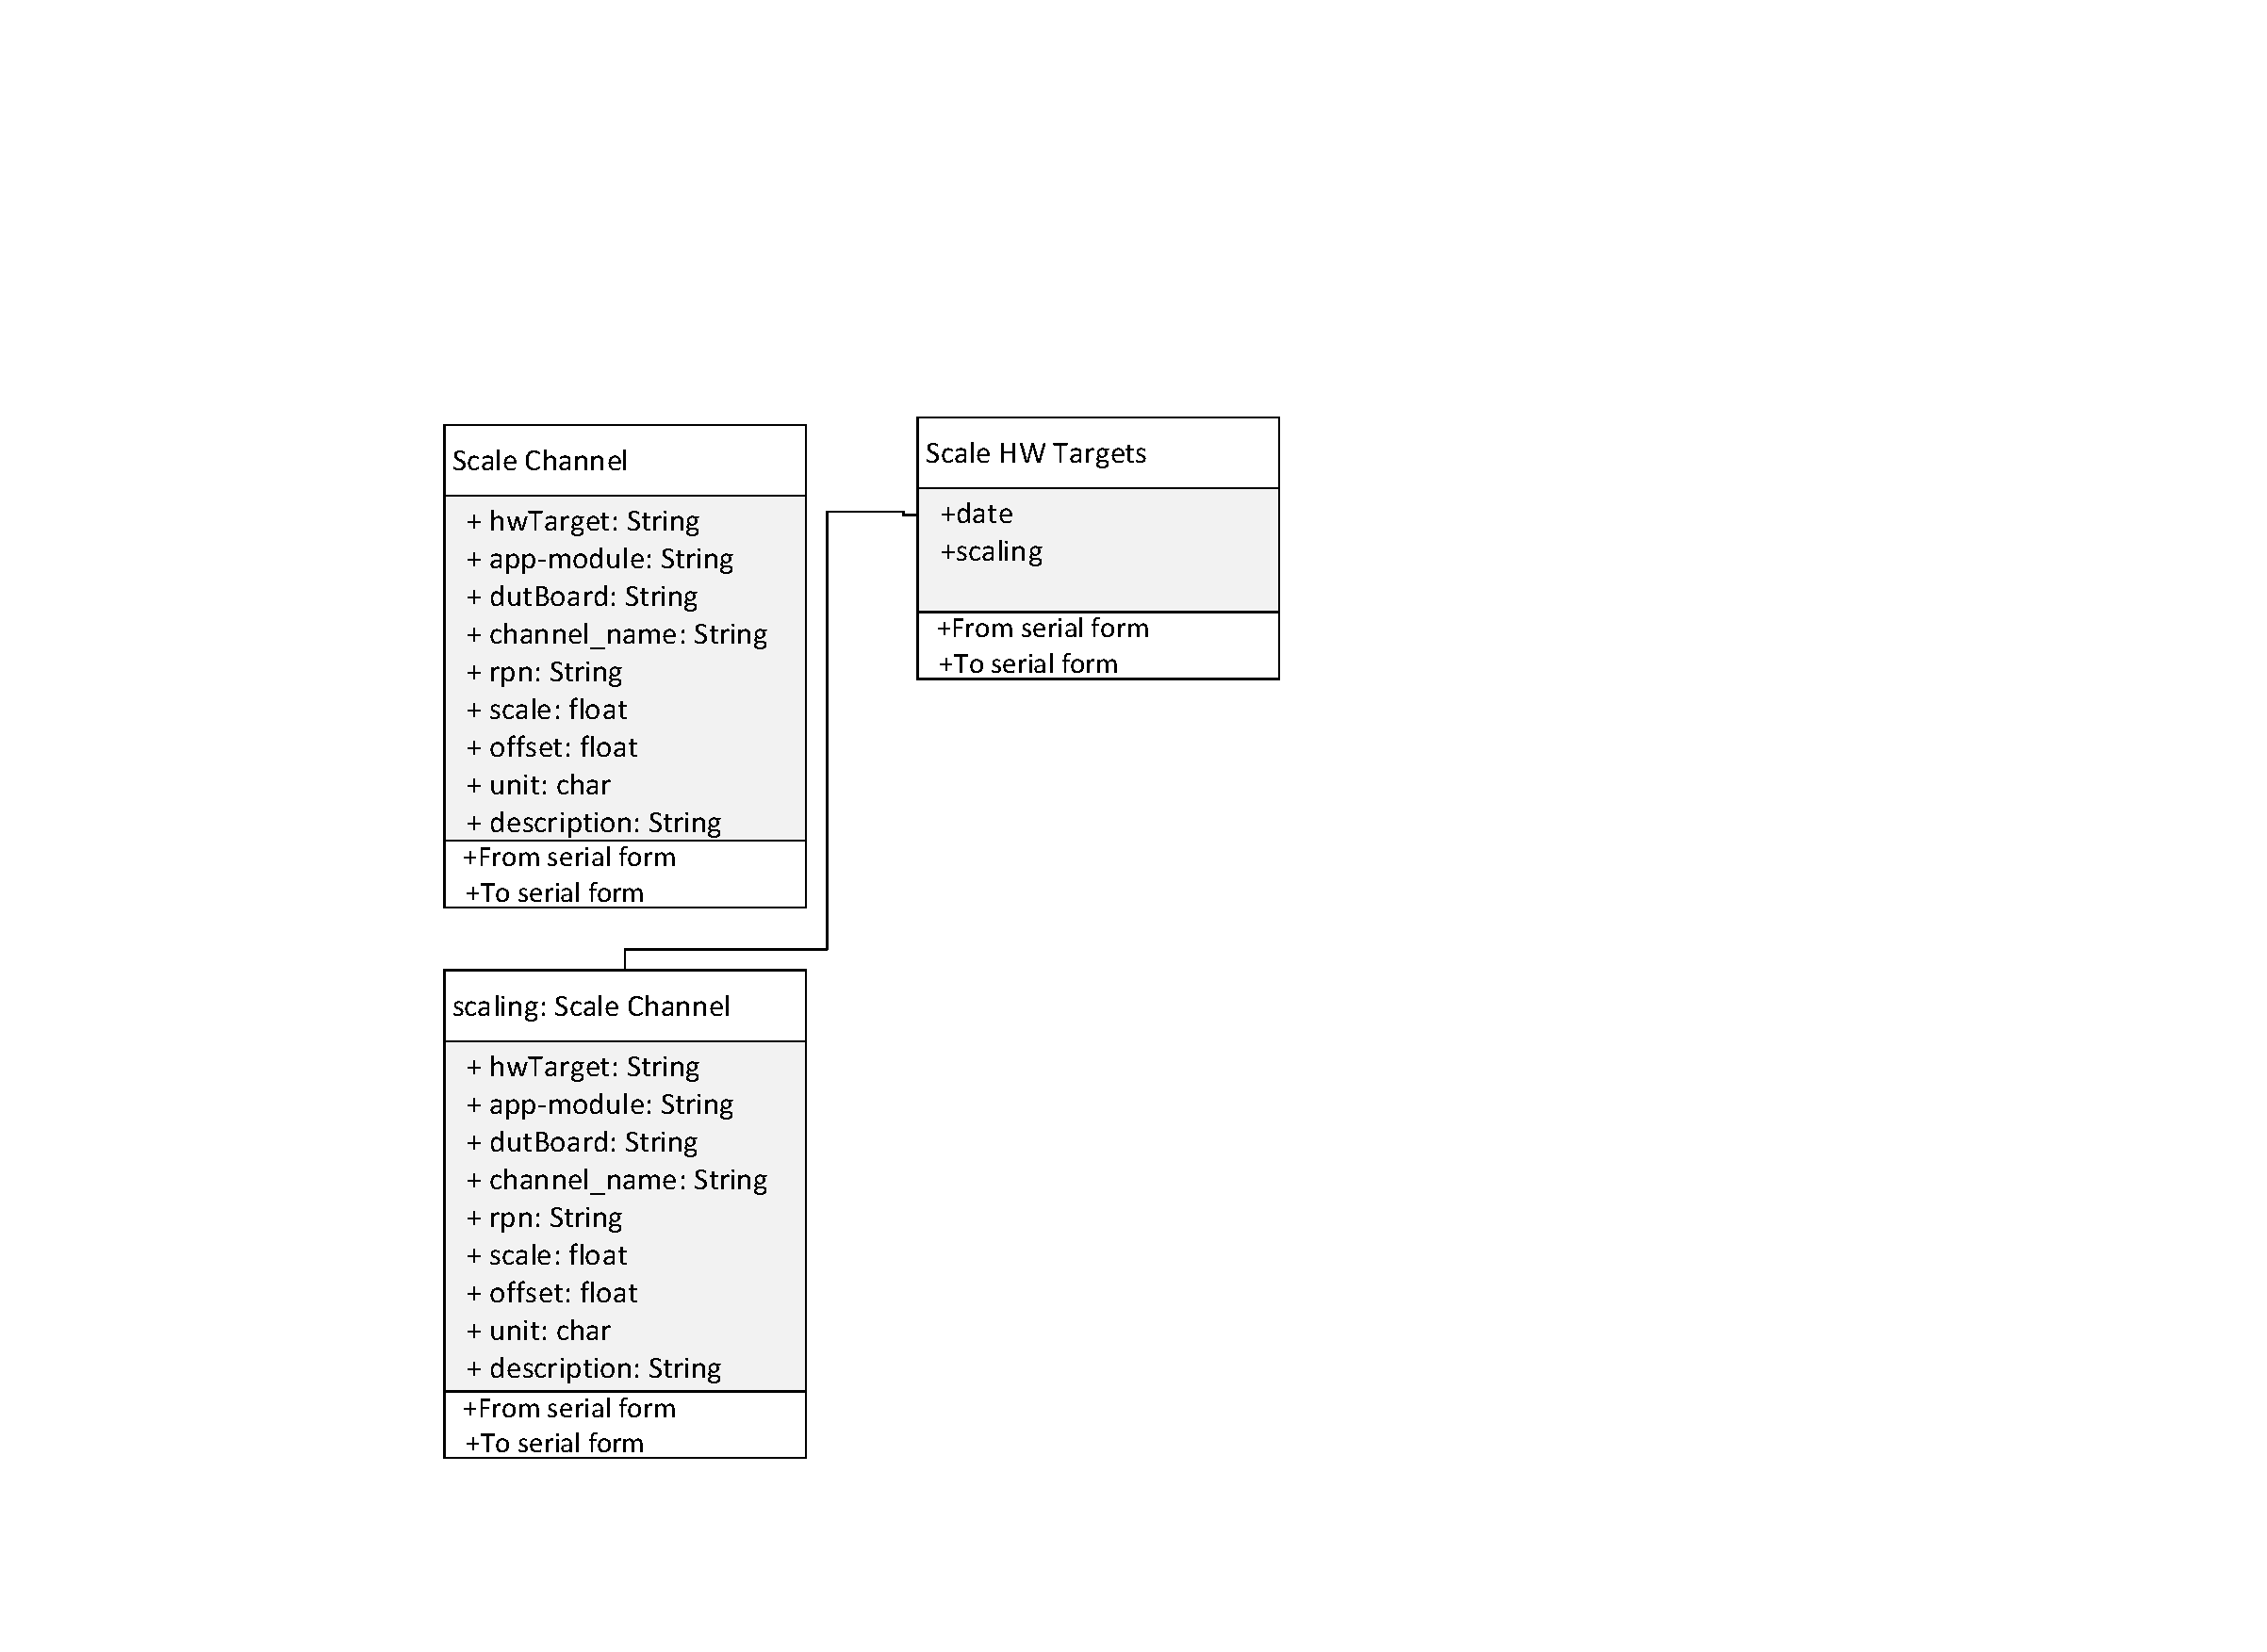
\includegraphics[trim=0 55 0 210, clip, width=210mm, scale=0.75]{images/Scaling_channel.pdf}
		\caption{Serialization of "scaling.json" objects into LabVIEW data structures}
		\label{fig:scSerialization}
\end{figure}

After successful verification, the board names correspondent combination is searched from the "Scale HW Targets" LabVIEW object. 
"Scaling" object is a result of serialization of "scaling.json" (\cref{fig:Communication}) into LabVIEW objects.
Serialization of "scaling.json" (\cref{fig:Communication}) into LabVIEW objects enables the conversion of JSON objects (\cref{lst:scaling}) present in the "scaling.json" into strings. 
After Serialization, filtering of channel names, scaling values and offset parameters, and communication of the same are done at a particular sequence as shown in the \cref{fig:Communication}. 
Below are the operations that are done at the mentioned sequence:       

\begin{enumerate}
\item Read the configuration path.
\item The text present in the text file is read.
\item De-serialization of JSON objects into LabVIEW objects is performed.
\item The data members of the "Scaling" object i.e Hardware Target, application module and \acrshort{DUT} board combination are compared with the applicationModule and dutModule objects. 
In the case of successful match, the board combination specific scaling value, offset and channel name are filtered from the "Scaling" object. 
The filtered parameters are further communicated to the board ID receiver handler~\cite{Steinwender2016} of MicroMoPS. 
\end{enumerate}

\begin{figure}[hbt]
		\centering
		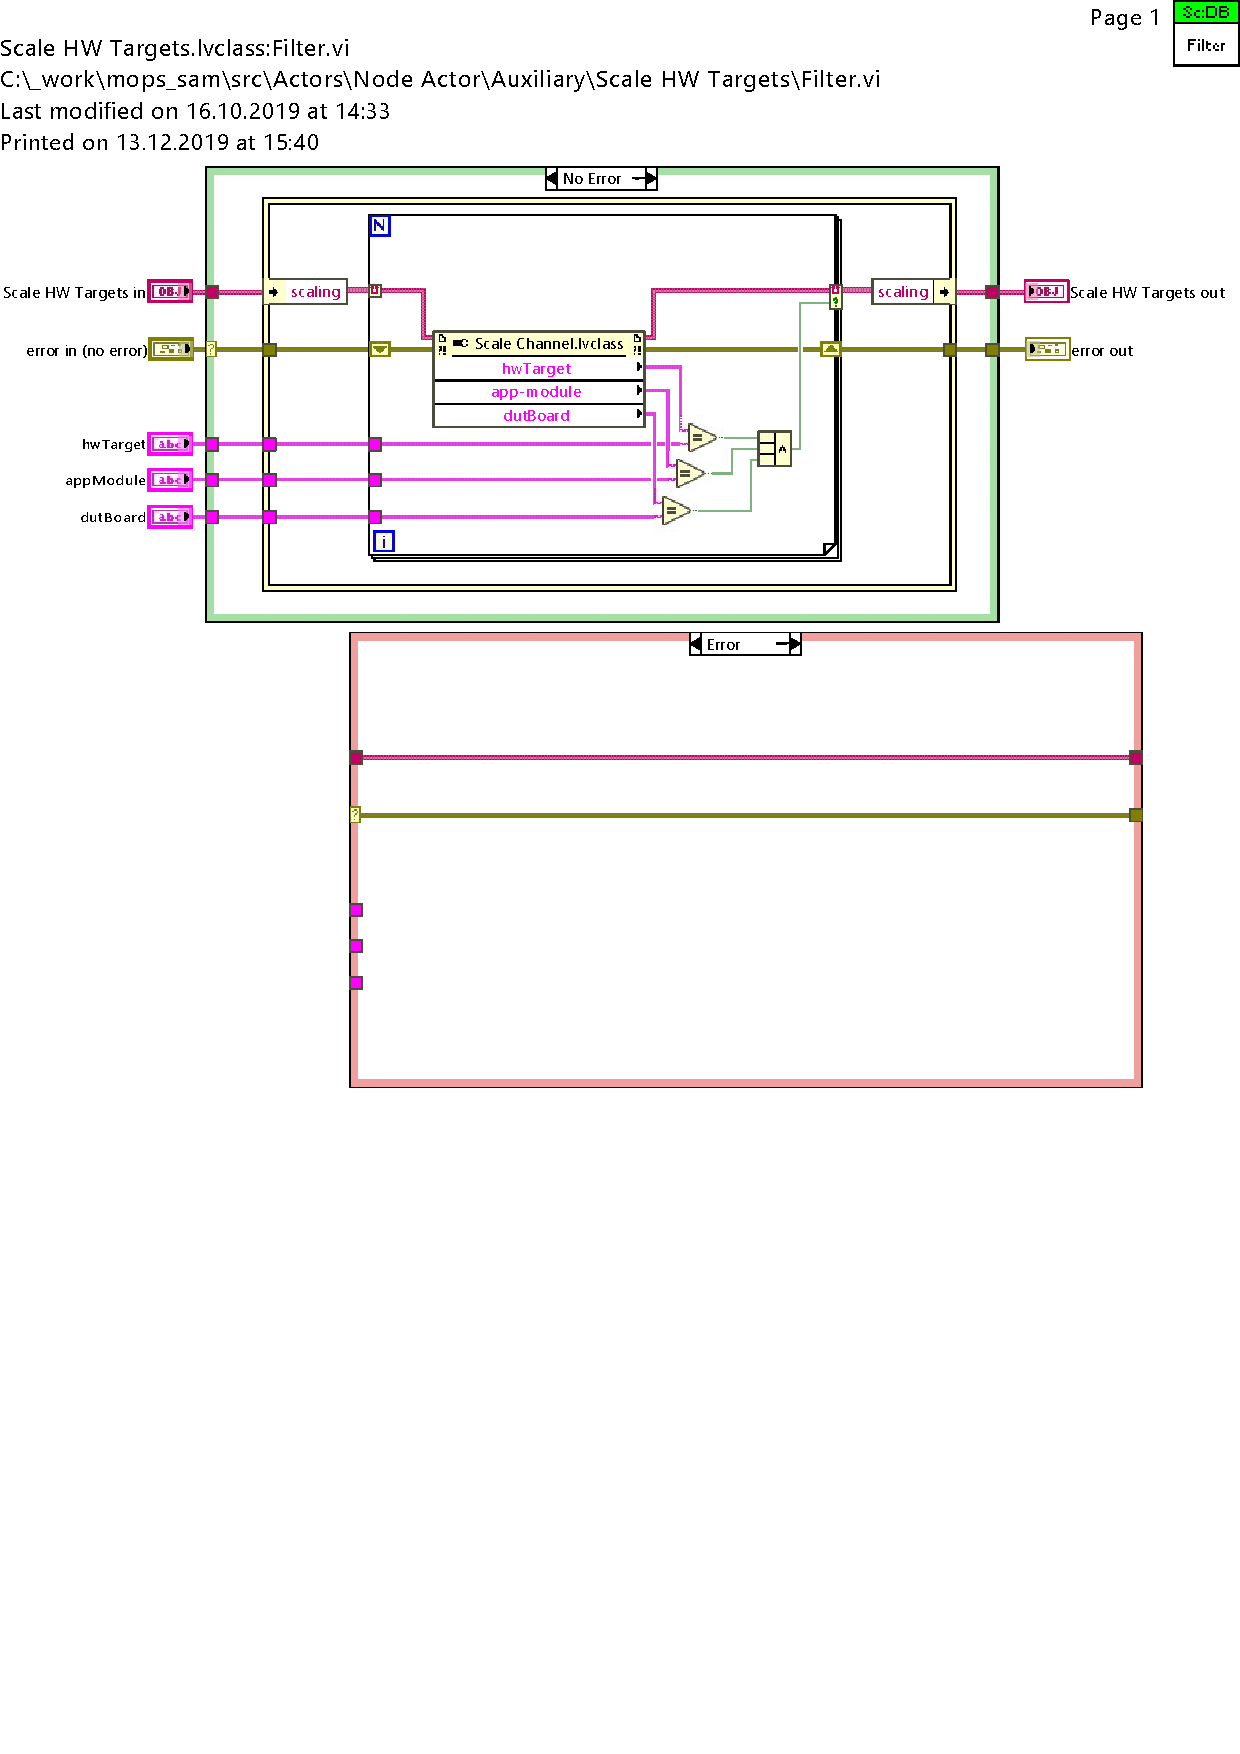
\includegraphics[trim=0 540 0 75, clip, width=130mm, scale=0.75]{images/filterVI.pdf}
		\caption{Filtering of scaling values}
		\label{fig:FOS}
\end{figure}

The filtering of the scaling values are implemented as shown in the \cref{fig:FOS}. 
The "Scaling" object is an instance of "Scale Channel" class which contains the hwTarget, app-module, 
dutBoard, channel\_name, rpn, scale, offset, unit and description data members. 
Data members such as scale, offset and channel\_name are filtered by performing a comparison between the board names that are obtained after resolution and the hwTarget, app-module and dutBoard data members, respectively. 
The control module's board name is obtained from the hardware information present in \acrshort{EDS}.   

\begin{figure}[hbt]
		\centering
		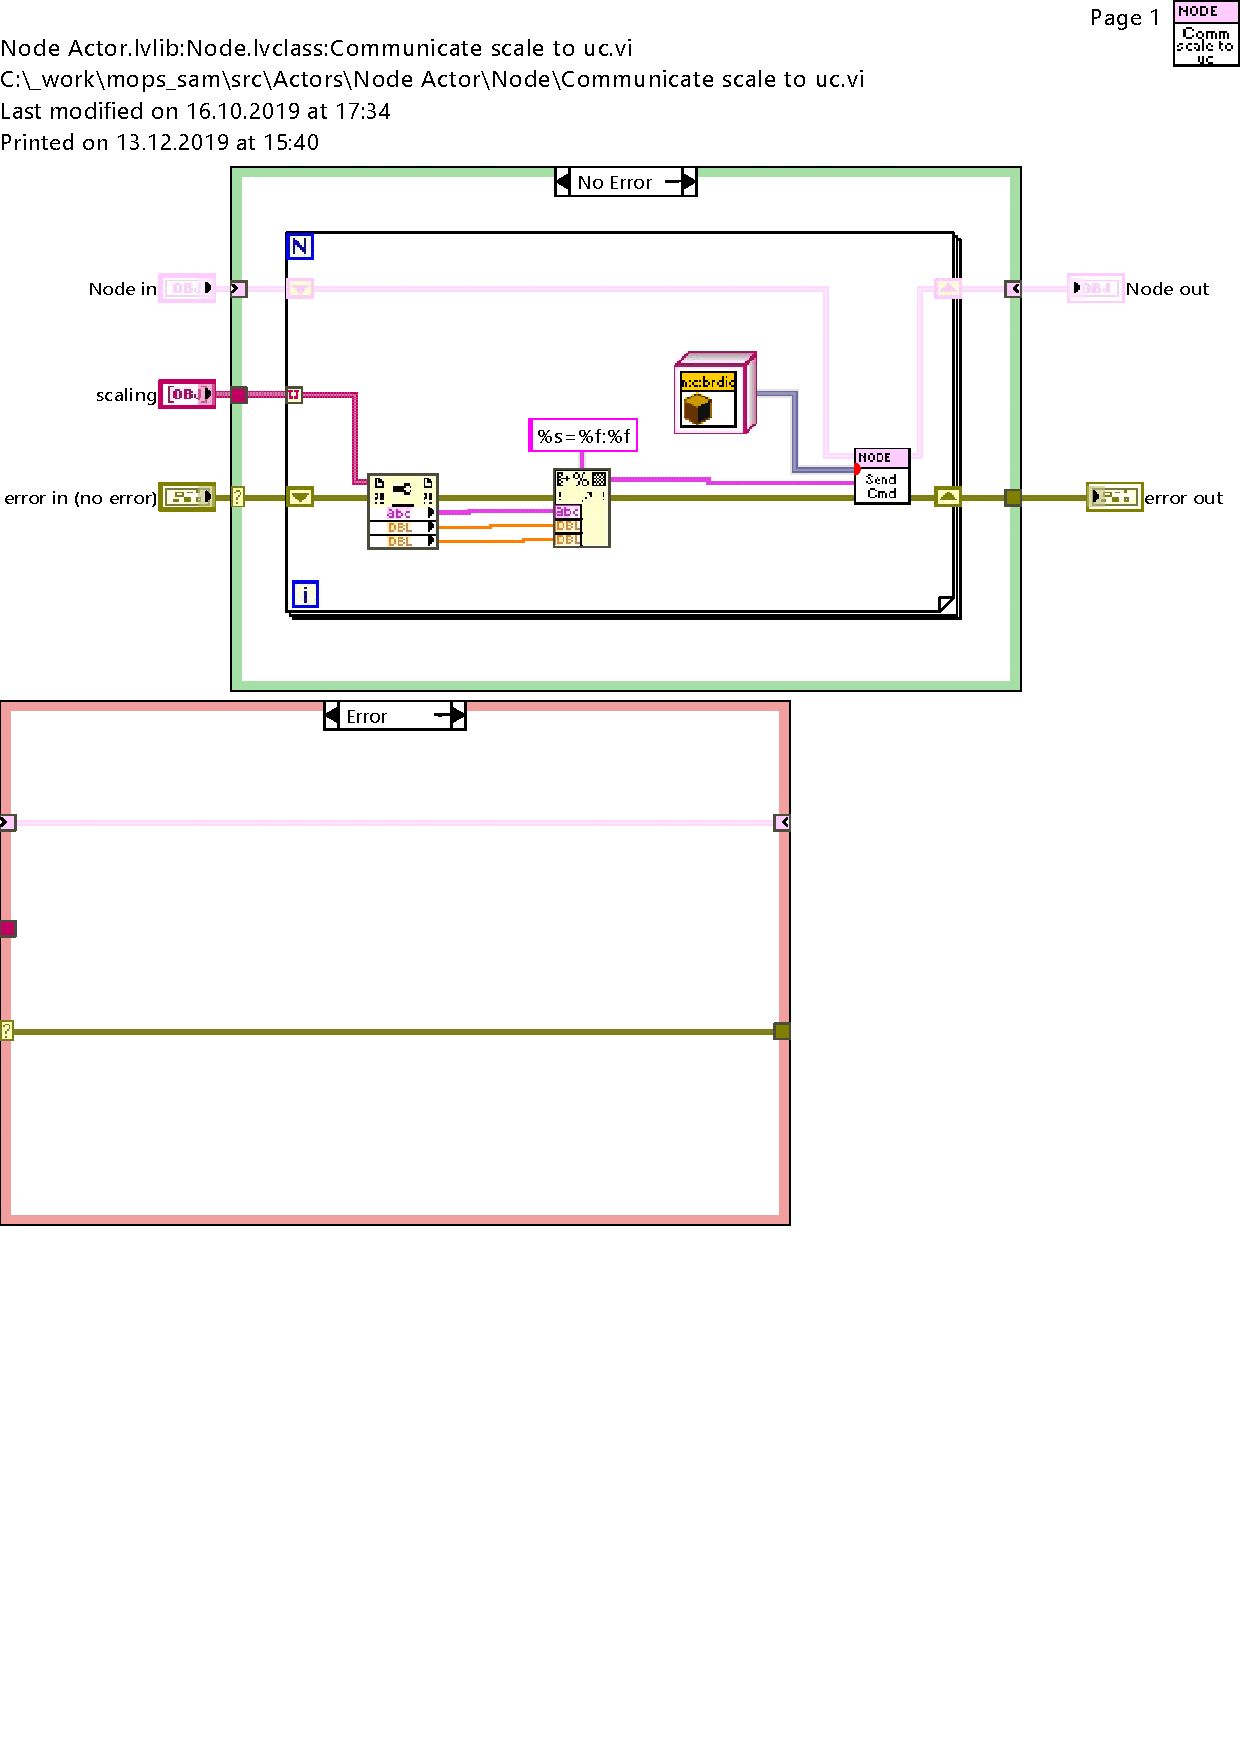
\includegraphics[trim=0 510 0 75, clip, width=130mm, scale=1]{images/commscaling.pdf}
		\caption{Communication of scaling values}
		\label{fig:COS}
\end{figure}


Finally, the filtered parameters are communicated to the board ID receiver handler of MicroMoPS. 
The filtered parameters are specific to every individual channel. 
The parameters are channel-wise communicated in a queue to MicroMoPS.
The \acrshort{VI} implementation of communication of scaling values is as shown in the \cref{fig:COS}.   

\section{Parse the scaling parameters dynamically in MicroMoPS}\label{sec:parse}
	Sequentially, the board combination specific communication channels and their respective scaling parameters are received as a payload (string data) from \gls{SAM} to board ID receiver handler (MoPS\_cmd\_handler\_BOARDID()) of MicroMoPS (see \cref{fig:DP}). 
	The string data that is obtained at board ID receiver handler of MicroMoPS is delimited by ':' between channel name and scaling parameters. It as shown in the example: "sync0:0B:0.0007326007326:0". 
	Where, sync0:0B is a channel name and module (see \cref{sec:Channels}), 0.0007326007326 is a value of the scaling factor denoted by 'k' and 0 is a value of offset denoted by 'd'. 
	This string is dynamically parsed and assigned to channel-specific scale (.scale) and offset (.offset) variables (see \cref{fig:DP}) present in the "MoPSscaling" module.
	Other parameters such as .func and .name are presesnt in order to define the RPN function and the communication channel module, respectively. These parameters are globally used in MoPS firmware, which are defined in the configuration file of MoPS firmware.   
	At present, the RPN string corresponding to the communication channels is not communicated from SAM.	  

\begin{figure}[hbt]
		\centering
		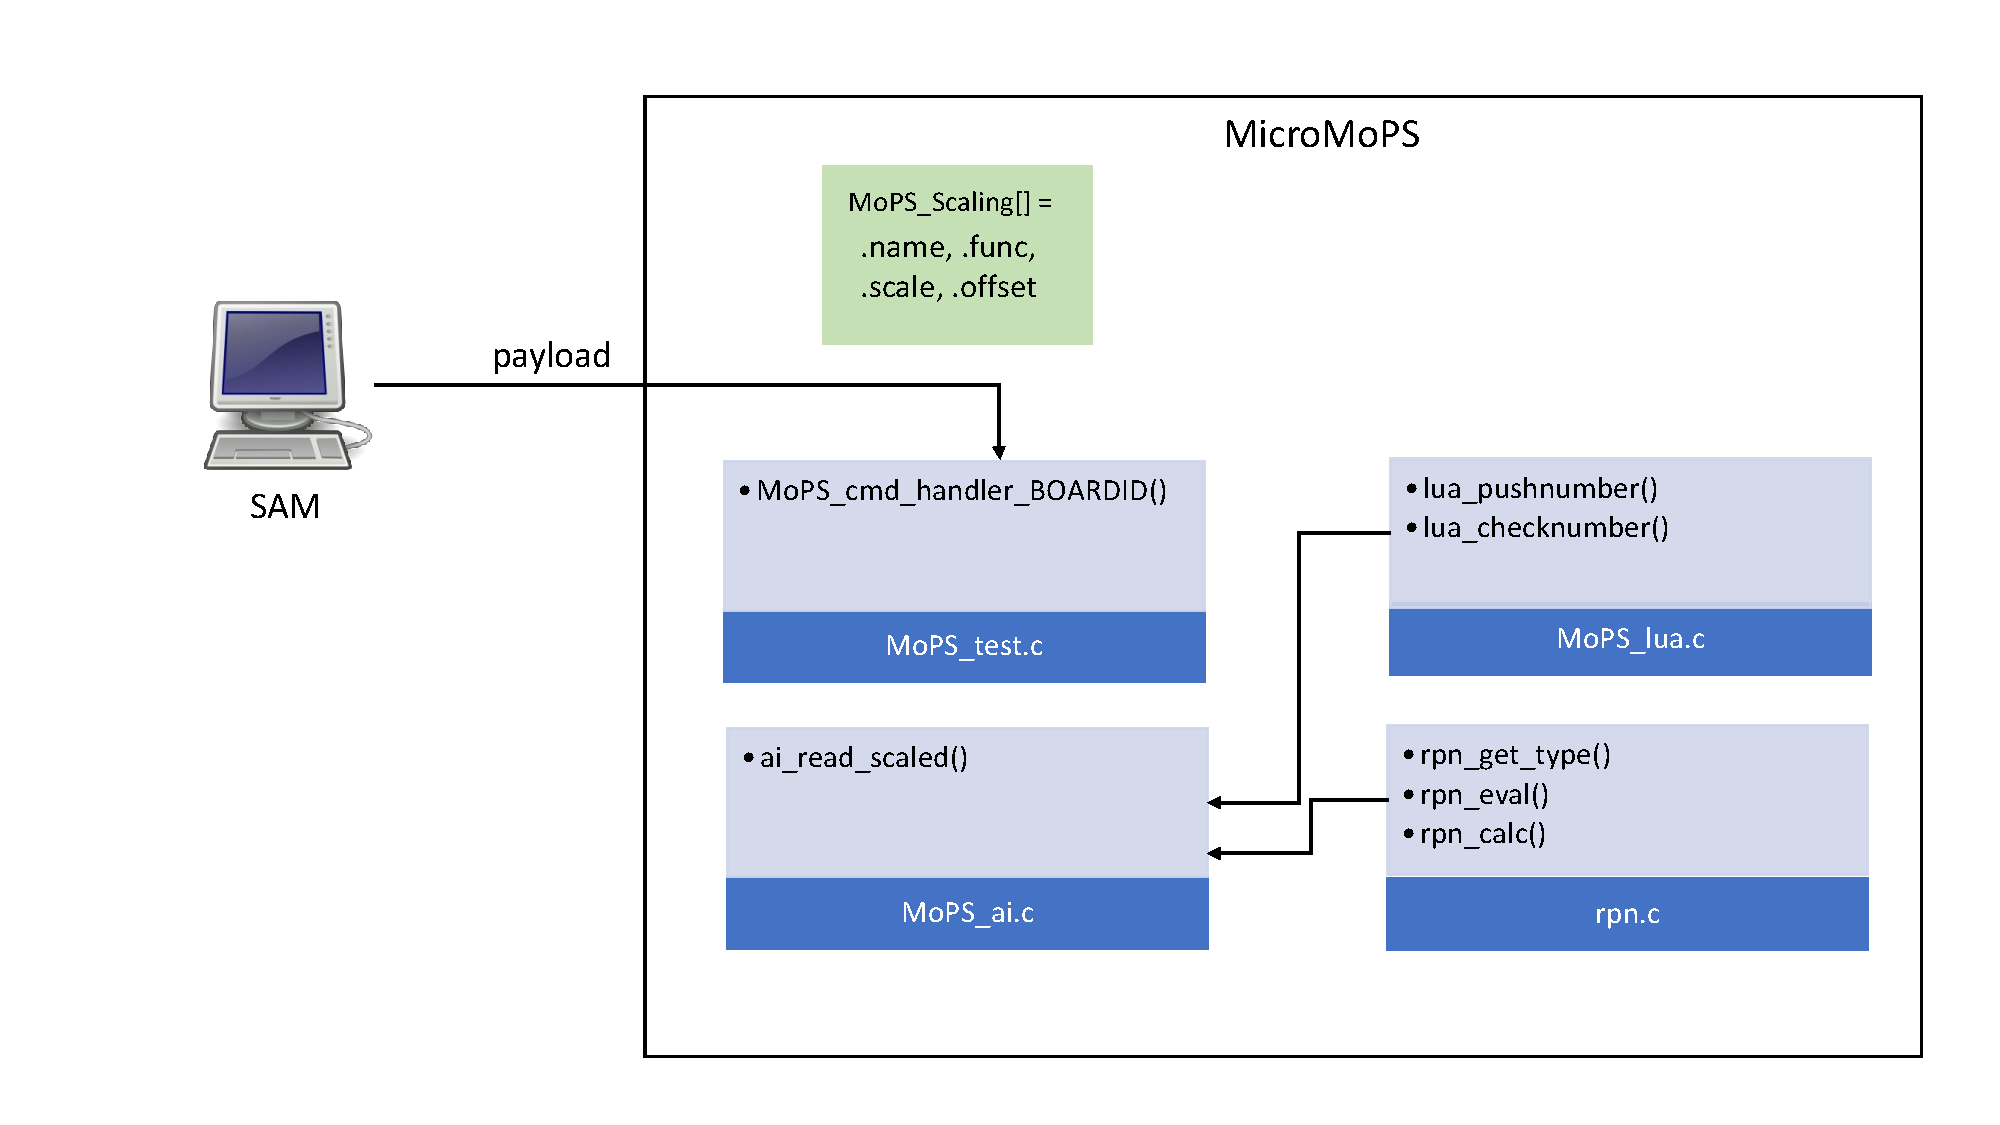
\includegraphics[trim=50 30 0 0, clip, width=152mm, scale=1]{images/Scaling_implementation.pdf}
		\caption{Implementation of data processing module}
		\label{fig:DP}
\end{figure}

\section{Compute scaling mechanisms in MicroMoPS}\label{sec:scaling}
	 In this work, linear scaling formula (see \cref{sec:linear function}) and Reverse Polish notation (see \cref{sec:RPN}) are implemented within the Lua handler of analog input module of MicroMoPS. 
	 The linear scaling formula uses the updated scaling parameters to process the analog measurements. 
	 RPN computation is achieved by making use of three fundamental handlers, such as `rpn\_get\_type()',
	 `rpn\_eval()' and `rpn\_calc()'. These handlers are defined in the `rpn.c' file (see \cref{fig:DP}). 
	 The `rpn\_get\_type()' handler is meant for decoding the respective operations or tokens based on the string data that is received from the SAM. The allowed operations in the RPN module are float variables, addition, subtraction, multiplication, division, square root, minimum function, and maximum function.
	 From the decoded type the respective operation is performed through the `rpn\_eval()' handler. The `rpn\_calc()' handler makes use of `rpn\_get\_type()' and `rpn\_eval()' handlers to perform the RPN computation. Along with the mentioned handlers the `rpn\_calc()' handler makes use of some of the functions that are part of Lua interpreter to memory efficiently (see \cref{sec:RPN}) perform the RPN computation. Finally, the MoPS\_scaling module (ai\_read\_scaled()) makes use of either `rpn\_calc()' or linear scaling formula to process the data using dynamically parsed scaling parameters (see \cref{sec:parse}).  
The operation of the RPN scaling mechanism is tested by hard coding the RPN string (see \cref{sec:RPN}) to channel-specific .func variable (updated in the config file).
Hard coding of RPN string is achieved by communicating the RPN string from TinyHost to MicroMoPS.